% \VignetteIndexEntry{An R Package for the Naive Bayes document classification in Java}
% \VignetteDepends{JNaiveBayes}
% \VignetteKeyword{Naive Bayes, Java, Poisson}



\documentclass[a4paper]{article}
\addtolength{\oddsidemargin}{-.875in}
\addtolength{\evensidemargin}{-.875in}
\addtolength{\textwidth}{1.75in}
\addtolength{\topmargin}{-.875in}
\addtolength{\textheight}{1.75in}
\usepackage{graphicx}
\usepackage{amsmath}
\usepackage{cases}
\usepackage{amsfonts}
\usepackage{bbm}
\usepackage{amssymb}

\usepackage{Sweave}
\begin{document}
\title{`JNaiveBayes` package}
\author{Tyler Olson \and Alex Zajichek}
\date{\today}
\maketitle
\abstract{The {\tt JNaiveBayes} package implements a Naive Bayes' text classifier with a very direct approach of allowing the user to supply directories of documents containing words, and receive predicted classifications of unclassified test documents. The user has the option to use a parametric approach, which uses a Poisson distribution on word counts, or a nonparametric approach, which calcaluates probabilities based on observed proportions. An additional tuning parameter is also available for each formulation, giving the user the option to weight unobserved words as seen fit. The heavy computation is done in a collection of Java classes by using the {\tt rJava} package as an interface within the {\tt JNaiveBayes} function. The goal of this project was to explore R's capabilities' to connect with Java, and to successfully build an R package using the connection.}

\section{Introduction}
Classification in the field of machine learning is used to predict some type of categorial response for individual observations. The supervised classification of text, where labeled data is used to train the model, has a wide range of applications. Spam detection, word comprehension, and genre identification are just a few examples of the utility of text classification. This paper will develop a Naive Bayes text classifier in two model formulations: parametric, and nonparametric. The models will then be implemented in Java, interfaced by R with the {\tt rJava} package, and combined into a single R package for user accessibility. The user will be able to supply documents with the purpose of categorizing new ones.
\section{Model Formulation}
 
Let 
\begin{itemize}
\item $C_i$ be the $i^{th}$ document category where $i=1,2,...,K$  
\item $D_j$ be the $j^{th}$ document where $j =1,2,...,M_i$
\item $W_{jk}$ be the $k^{th}$ {\it unique} word in $D_j$ where $k=1,2,...,N_j$  
\item $O_{jk}$ be the {\it occurrence} of $W_{jk}$ in $D_j$ 
\end{itemize}
The Na\"{i}ve Bayes' model can then be defined in two formulations:
\subsection*{Parametric}
Let 
$$O_{jk}|C_i \sim Poisson(\lambda_{ik} = \frac{\sum_{j=1}^{M_i} O_{jk}}{M_i} )$$
where $\lambda_{ik}$ is the average occurrence of word $W_{jk}$ in $M_i$ documents of a given category, and
$$C_i \sim Bernoulli(p_i = \frac{M_i}{\sum_{i'=1}^K M_{i'}})$$
where $p_i$ is the proportion of total documents belonging to category $i$. Then, \\

\begin{align*}
P(C_i | D_j) & \propto P(D_j | C_i)P(C_i) \\
& = P(O_{j1}^* \cap O_{j2}^* \cap ... \cap O_{jN_j}^* | C_i)P(C_i) \\
& = P(O_{j1}^*|C_i)P(O_{j2}^*|C_i) \times ... \times P(O_{jN_j}^*|C_i) P(C_i) \\
& = \prod_{k=1}^{N_j} P(O_{jk}^*|C_i) P(C_i) 
\end{align*}
where 

\begin{align*}
P(O_{jk}^*|C_i) & = (1-\delta)\frac{P(O_{jk}|C_i)}{P(O_{jk} > 0|C_i)} +  \frac{\delta}{\sum_{j=1}^{M_i} \sum_{k=1}^{N_j} O_{jk}} \\
 & = (1-\delta)\frac{e^{-\lambda_{ik}}\lambda_{ik}^{O_{jk}}}{O_{jk}!(1-e^{-\lambda_{ik}})} +  \frac{\delta}{\sum_{j=1}^{M_i} \sum_{k=1}^{N_j} O_{jk}} \\
\end{align*}
and $\delta$ is a smoothing parameter that allows a small-weighted positive probability to be assigned to unobserved words in a category.


\subsection*{Nonparametric}
The nonparametric approach calculates probabilities based on proportions of word occurences. Let
$$P(C_i) = \frac{M_i}{\sum_{i'=1}^K M_{i'}}$$
and 
$$P(W_{jk} | C_i) = (1-\delta)\frac{\sum_{j=1}^{M_i} O_{jk}}{\sum_{j=1}^{M_i} \sum_{k=1}^{N_j} O_{jk}} +  \frac{\delta}{\sum_{j=1}^{M_i} \sum_{k=1}^{N_j} O_{jk}}$$ 
where $M_i$ is the number of documents in category $i$. Then,
\begin{align*}
P(C_i | D_j) & \propto P(D_j | C_i)P(C_i) \\
& = P(W_{j1}|C_i)^{O_{j1}}P(W_{j2}|C_i)^{O_{j2}} \times ... \times P(W_{iN_j}|C_i)^{O_{jN_j}} P(C_i) \\
& = \prod_{k=1}^{N_j} P(W_{jk}|C_i)^{O_{jk}} P(C_i) \\ 
\end{align*}

\noindent Therefore, given a new document,
$$P(C_i|D_j) = \frac{P(D_j|C_i)P(C_i)}{\sum_{i=1}^K P(D_j|C_i)P(C_i)}$$
can be computed in both model specifications.

\subsection{More on $\delta$}
The difference in probability calculation between the parametric and nonparametric approaches is only present for words in a document that have been previously observed by a category. If the word has not been observed, a probability of one over the total number of words in a category is given. Further, the $\delta$ parameter allows the user the freedom to weight these unobserved words as seen fit. Typically it should be a small value. By default, $\delta = 0.01$.

\section{Requirements}
\subsection{Data}
Due to certain coding decisions that were made during the development process, the text files composing of the training and testing sets must follow a particular structure. The BufferedReader class in Java is used to read an input stream line-by-line from each text file, and the line is not parsed before it is stored within a hash map. Therefore, each text file must be newline delimited. If a certain training document consists of 30 words for example, each of the 30 lines in the text file should only contain a single word and there should be no punctuation or additional white space. Characters such as apostrophes and hyphens that contribute to a word's meaning should be preserved. 
\subsection{Directory}
The data for this package should be stored according to a specific directory structure. The training and testing sets must be located in separate folders. For example, the training instances could be stored in the ``Training" directory, while the test cases could be stored in a ``Testing" directory. The ``Testing" directory would only contain the unlabeled test documents. The ``Training" folder would contain subdirectories for each of the relevant grouping categories. Each subdirectory would contain the training documents belonging to the respective category or class. For example, suppose a user was interested in classifying an email as public or private. If they had 100 known public emails in their training set, these 100 emails would be stored in a ``public" subdirectory within the ``Training" directory.
\section{Example}
\begin{Schunk}
\begin{Sinput}
> library(JNaiveBayes)
> library(xtable)
> train <- system.file("Data", "Training", package = "JNaiveBayes")
> test <- system.file("Data", "Testing", package = "JNaiveBayes")
> model1 <- JNaiveBayes(trainDir = train, testDir = test, parametric = FALSE, delta = 0.01)
> model2 <- JNaiveBayes(trainDir = train, testDir = test, parametric = TRUE, delta = 0.01)
> model3 <- JNaiveBayes(trainDir = train, testDir = test, parametric = FALSE, delta = 0.15)
> xtable(model1$Probabilities);xtable(model2$Probabilities);
\end{Sinput}
% latex table generated in R 3.3.3 by xtable 1.8-2 package
% Wed May  3 20:48:40 2017
\begin{table}[ht]
\centering
\begin{tabular}{rrr}
  \hline
 & Personal & Public \\ 
  \hline
unknown1.txt & 0.10 & 0.90 \\ 
  unknown2.txt & 0.97 & 0.03 \\ 
  unknown3.txt & 1.00 & 0.00 \\ 
   \hline
\end{tabular}
\end{table}% latex table generated in R 3.3.3 by xtable 1.8-2 package
% Wed May  3 20:48:40 2017
\begin{table}[ht]
\centering
\begin{tabular}{rrr}
  \hline
 & Personal & Public \\ 
  \hline
unknown1.txt & 0.75 & 0.25 \\ 
  unknown2.txt & 1.00 & 0.00 \\ 
  unknown3.txt & 1.00 & 0.00 \\ 
   \hline
\end{tabular}
\end{table}\end{Schunk}

\section{Application}
This section gives a demonstration of the {\tt JNaiveBayes} package for a publicly available dataset found at the following website:
\begin{center}
{\footnotesize{
\begin{verbatim}
https://www.kaggle.com/crowdflower/twitter-airline-sentiment
\end{verbatim}}}
\end{center}
The goal of this application will be to test the predictive ability of this methodology in regards to {\it sentiment analysis}. Given a number of sentiments (categories) and their corresponding documents, a large test set will be classified. The test set will be held out of the original data so the number of correct classifications can be obtained. The R code used will be included.

\subsection{Data description}
The archive from the webpage contains Twitter information of many users' ``tweets" towards a number of US airlines from 02/16/2015-02/24/2015. There are a total of 14640 recorded tweets in the dataset, each with one of the corresponding sentiments: {\it negative, neutral, positive}. Below shows the first 3 rows of the dataset, after removing everything but the tweets and labels, including punctuation:
{\footnotesize{
\begin{verbatim}
> tweets <- read.csv("Tweets.csv", header = T, stringsAsFactors = FALSE)
> tweets <- data.frame("Sentiment" = as.character(tweets$airline_sentiment), 
+ "Tweet" = gsub("[[:punct:]]",'',as.character(tweets$text)))
> head(tweets)[1:3,]
  Sentiment                                                              Tweet
1   neutral                                   VirginAmerica What dhepburn said
2  positive VirginAmerica plus youve added commercials to the experience tacky
3   neutral  VirginAmerica I didnt today Must mean I need to take another trip
\end{verbatim}}}
\noindent We will randomly select 1000 tweets to be held out for classification, leaving 13640 to build the model.
{\footnotesize{
\begin{verbatim}
> set.seed(10) #For reproducibility
> test_inds <- sample(1:nrow(tweets),1000, replace = F)
> train <- tweets[-test_inds,]
> test <- tweets[test_inds,]
\end{verbatim}}}

\subsection{Data preprocessing}
Since all of this data is currently in a data frame, there needs to be some manipulation done to get it into the correct form for {\tt JNaiveBayes}, as described in the previous section. Each category must have its own directory, containing text files that have a single word on each line. Within each category, a separate file must be written out if the parametric approach is desired, since the Poisson mean depends on the count of documents in a category. The nonparmetric model, however, only needs a single document for each category, but will work the same regardless. For best practice, each document should get its own file. The following code was used to do this:
{\footnotesize{
\begin{verbatim}
> #separating out the three sentiments
> neut <- subset(train, Sentiment == 'neutral') 
> pos <- subset(train, Sentiment == 'positive')
> neg <- subset(train, Sentiment == 'negative')
>
> #Creating lists of tweets for each category
> neutral_tweets <- strsplit(neut$Tweet, ' ')
> negative_tweets <- strsplit(neg$Tweet, ' ')
> positive_tweets <- strsplit(pos$Tweet, ' ')
>
> #change directories so files write to correct place
> for(i in 1:length(neutral_tweets)) {
+    write.table(tolower(neutral_tweets[[i]][neutral_tweets[[i]] != ""]),
+                file = paste0("neutral",i,".txt"), row.names = F, quote = F, col.names = F)
+ }
> for(i in 1:length(negative_tweets)) {
+    write.table(tolower(negative_tweets[[i]][negative_tweets[[i]] != ""]),
+                file = paste0("negative",i,".txt"), row.names = F, quote = F, col.names = F)
+ }
> for(i in 1:length(positive_tweets)) {
+    write.table(tolower(positive_tweets[[i]][neutral_tweets[[i]] != ""]),
+                file = paste0("positive",i,".txt"), row.names = F, quote = F, col.names = F)
+ }
\end{verbatim}}}

\noindent The same can be done for the testing documents, where each tweet gets its own file, within a single directory.
{\footnotesize{
\begin{verbatim}
> #storing the true labels
> test_labs <- test$Sentiment
>
> #obtaining a list where each element contains a tweet 
> 	#separated by word into a vector
> test_tweets <- strsplit(as.character(test$Tweet), ' ')
>
> #looping through the list and writing each tweet to a file
> 	#each with a different name
> for(i in 1:length(test_tweets)) {
+    write.table(tolower(test_tweets[[i]][test_tweets[[i]] != ""]), 
+                file = paste0("tweet",i,".txt"), row.names = F, quote = F, col.names = F)
+ }
\end{verbatim}}}

\subsection{Obtaining predictions}
Once all preliminary work is finished, the model can be run.
{\footnotesize{
\begin{verbatim}
> library(JNaiveBayes}
> model <- JNaiveBayes(trainDir = "Sentiments", testDir = "TestTweets", delta = 0.01, parametric = FALSE)
> head(model$Probabilities)
                neutral     positive  negative
tweet1.txt 8.866285e-01 7.128072e-03 0.1062434
tweet2.txt 8.252757e-02 1.516138e-04 0.9173208
tweet3.txt 2.712118e-01 1.198543e-03 0.7275897
tweet4.txt 3.971737e-05 2.331257e-04 0.9997272
tweet5.txt 5.881125e-02 2.134934e-01 0.7276953
tweet6.txt 7.170408e-05 1.849576e-08 0.9999283
> preds <- apply(model$Probabilities, 1, which.max)
> labels <- colnames(model$Probabilities)[preds]
> correct <- as.numeric(labels == test_labs)
> mean(correct) #0.752
>
> #checking the time it takes to carry out the analysis
> system.time(JNaiveBayes(trainDir = "Sentiments", testDir = "TestTweets", delta = 0.01, parametric = FALSE))
   user  system elapsed 
  1.710   0.321   5.407 
\end{verbatim}}}
\noindent When using the default settings of the function, the model correctly classified 752 of the 1000 tweets in the testing data. This process took a total of 5.41 seconds to read in and store 13460 text files and calculate category probabilities for 1000 test documents.

\subsection{Exploring the tuning parameter}
The effect of the the choice of $\delta$ can be assessed by examing the classification rate at a range of values.
{\footnotesize{
\begin{verbatim}
> correct_classifications <- function(delta, parametric) {
+    model <- JNaiveBayes("Sentiments","TestTweets", delta = delta, parametric = parametric)
+    preds <- apply(model$Probabilities, 1, which.max)
+    labels <- colnames(model$Probabilities)[preds]
+    correct <- as.numeric(labels == test_labs)
+    mean(correct)
+ }
> deltas <- seq(0.01, .99, .01)
> results <- sapply(deltas, correct_classifications, parametric = FALSE)
> results2 <- sapply(deltas, correct_classifications, parametric = TRUE)
> Method <- c(rep("Parametric",length(results2)), rep("Nonparametric", length(results)))
> res <- c(results2, results); d <- c(deltas, deltas)
> library(ggplot2)
> Model <- rep("Nonparametric", length(results))
> ggplot() + geom_line(aes(x = d, y = res, colour = Method)) + 
ylab("%Correct Classifications") + xlab("Delta") + 
ggtitle("US Airlines Sentiment Analysis with JNaiveBayes")

\end{verbatim}}}
\begin{center}
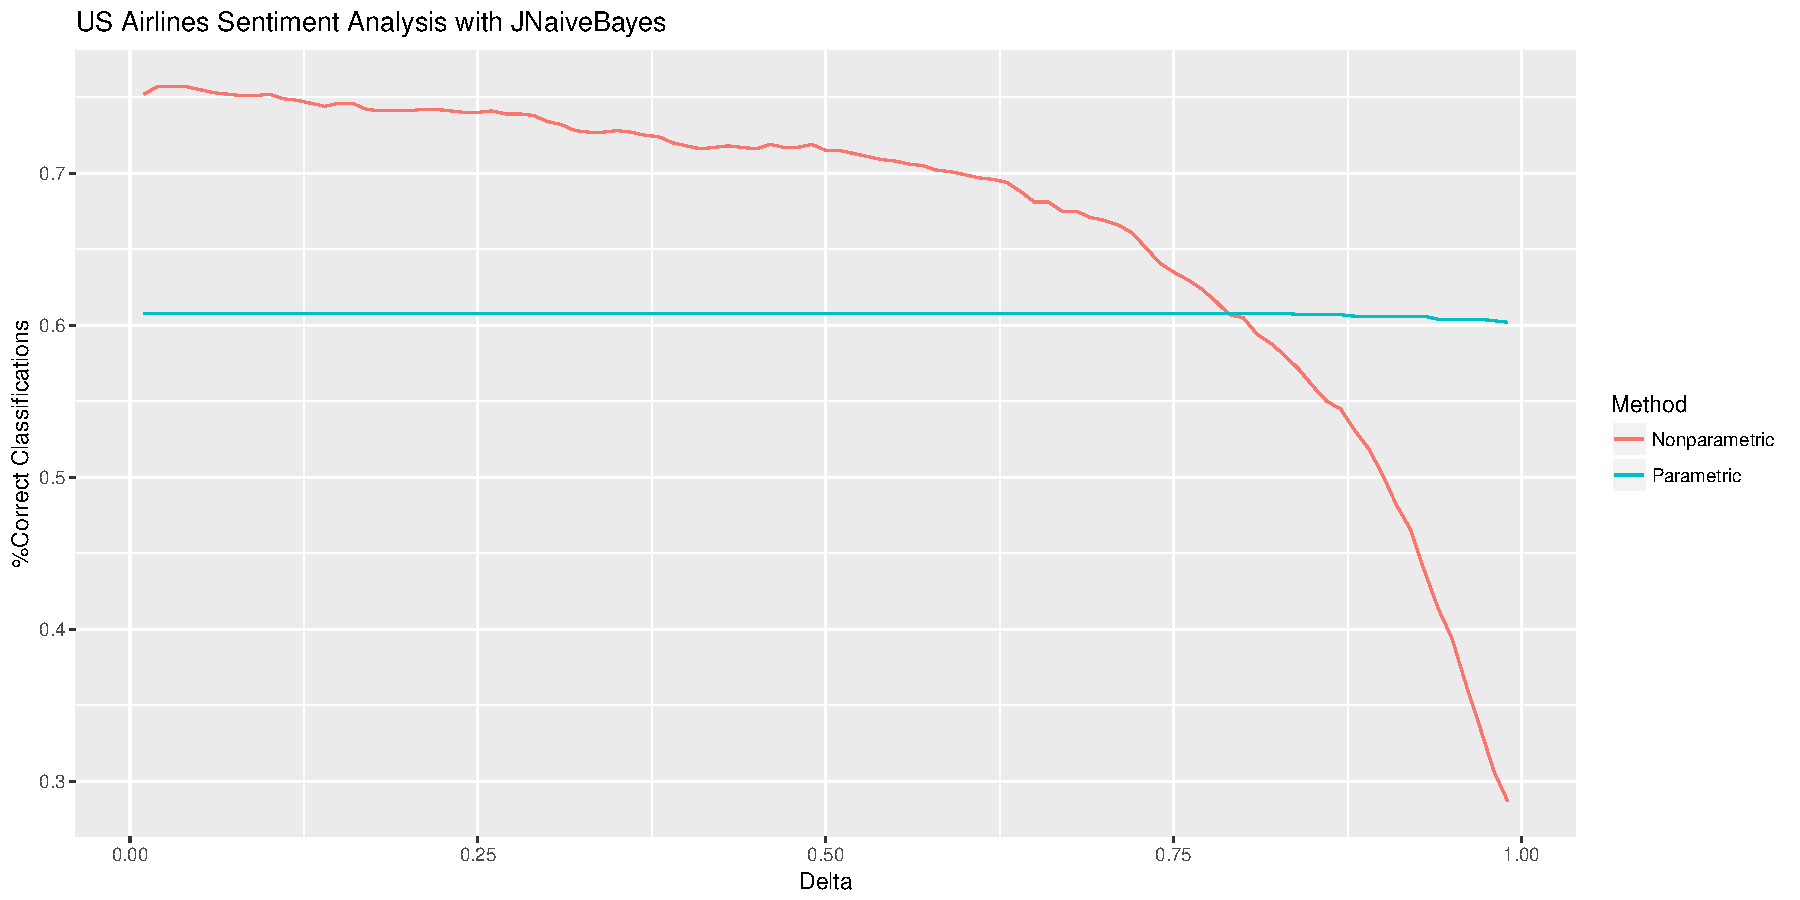
\includegraphics[scale=.6]{comparison.pdf}
\end{center}
The plot displays the proportion of correctly classified test documents for both parametric and nonparametric models on a range of $\delta$ values from (0,1). We observe that the choice of $\delta$ plays a significant role in the model's accuracy for the nonparametric approach, but had little impact on the parametric model.





\end{document}
